\documentclass[letterpaper, 12pt]{article}

\usepackage{graphicx}
\usepackage{longtable}
\usepackage{rotating}
\usepackage{dcolumn}
\usepackage{listings}
\usepackage{subfiles}
\usepackage{amsmath}

% Code listing commands
\lstset{language=R,
basicstyle=\scriptsize\ttfamily,
commentstyle=\ttfamily,
numbers=left,
numberstyle=\footnotesize,
stepnumber=1,
numbersep=5pt,
showspaces=false,
showstringspaces=false,
showtabs=false,
frame=single,
tabsize=2,
captionpos=b,
breaklines=true,
breakatwhitespace=false,
title=\lstname,
escapeinside={},
keywordstyle={},
morekeywords={}
}

\begin{document}
\title{ARE213 Problem Set \#2B}
\author{Peter Alstone \& Frank Proulx}
\maketitle

\section{Part A: Preliminaries}

\subsection{I: Comparison between TU and control States}

\paragraph{Starting with simple comparisons:}
We begin with simple comparisons between the dependent outcome of interest, the natural logarithm of traffic fatalities per capita (log(fatalities per capita)), between a predefined composite treatment state ``TU" (or, state \#99), and all of the potential control states.  The mean over the period before primary seatbelt laws were adopted in the treatment state is -1.4 and the mean for the control states is -1.7, indicating approximately a 30\% lower typical fatalities rate in the treatment state than the average control state (even before the primary seatbelt law ``treatment").  The trends for both shown in Figure \ref{fig:a11} show that overall the fatalities were on the decline in both places before the treatment period.  

\paragraph{Roadmap:}
Extracting meaningful conclusions from these data is the goal of our analysis, which will require identifying the variation in traffic fatalities that can be attributed to seat belt laws.  Confounding our analysis is the fact that these data are not in the context of an RCT but are from the ``real world" with messy trends and linked systems that determine outcomes.  We will be applying the synthetic controls method to identify a fleet of control states as a meaningful counterfactual to measure against for our composite treatment state.  

\begin{figure}[htbp]
\begin{center}
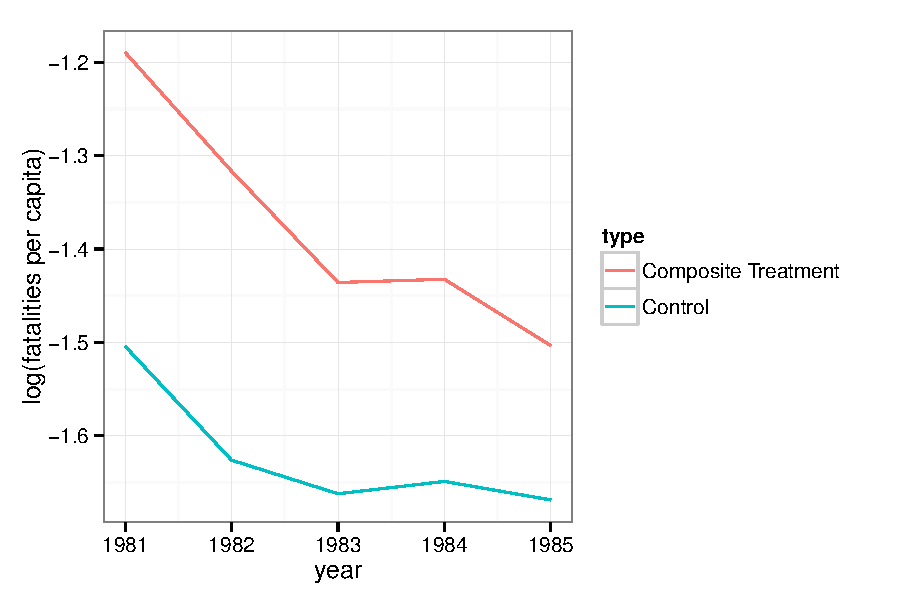
\includegraphics{img-p2b-logfatTrend.pdf}
\caption{Trend in the dependent variable (log(fatalities per capita)) for the composite treatment state and the average of the control states.}
\label{fig:a11}
\end{center}
\end{figure}


\subsection{II: ``Best" control state comparison}

\paragraph{Sweet Home Alabama:} 
We observe that Alabama is the best match for the composite treatment state based on a simple comparison of log(fatalities per capita) in the year before treatment in the composite state (1985).  Figure \ref{fig:a21} below shows the distribution in the dependent variable 

\paragraph{Fried green covariates and other stereotypes confirmed:}
Tables \ref{tab:a21} and \ref{tab:a22} compare the covariates for the composite treatment state and Alabama.  There are broad differences between the states.  Alabama has higher precipitation, lower college achievement, lower alcohol consumption, higher unemployment, etc.  Additionally, the mean value for the depdentent variable of interest, log(fatalities per capita), is quite different for the two states.  Examining the trends in the covariates (and dependent variable) for the two states (see Figure \ref{fig:a22}) shows that it could be construed as a coincidence that Alabama is the best match for the value of the dependent variable, since the trajectory in fatalities for both states are following opposite trends in that time and 1985 happens to be the time when they intersect.  There are also important and long-term differences in precipitation and alcohol consumption.  

Overall Alabama does not appear to be a particularly good match for the composite treatment state, motivating an application of synthetic controls methods to produce a better match.  

\begin{figure}[htbp]
\begin{center}
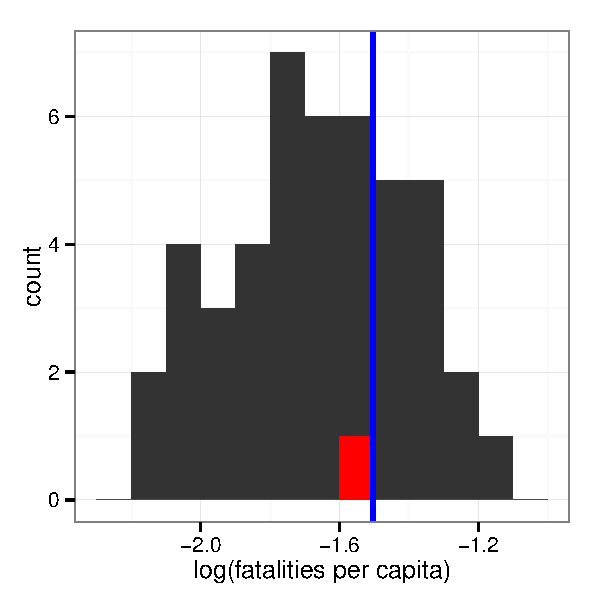
\includegraphics{img-p2b-compareStates.pdf}
\caption{Distribution in traffic fatalities metric from 1985 for all control states with a vertical blue line indicating the value of the metric for the composite treatment state.  The red block highlights the position of Alabama in the distribution.  Alabama is the closest match to the composite treatment state for 1985, but as is shown here is one of about 11 states that is within ~10\% of the target value.}
\label{fig:a21}
\end{center}
\end{figure}

\subfile{tab-ps2b-1a.tex}
\subfile{tab-ps2b-1b.tex}

\begin{figure}[htbp]
\begin{center}
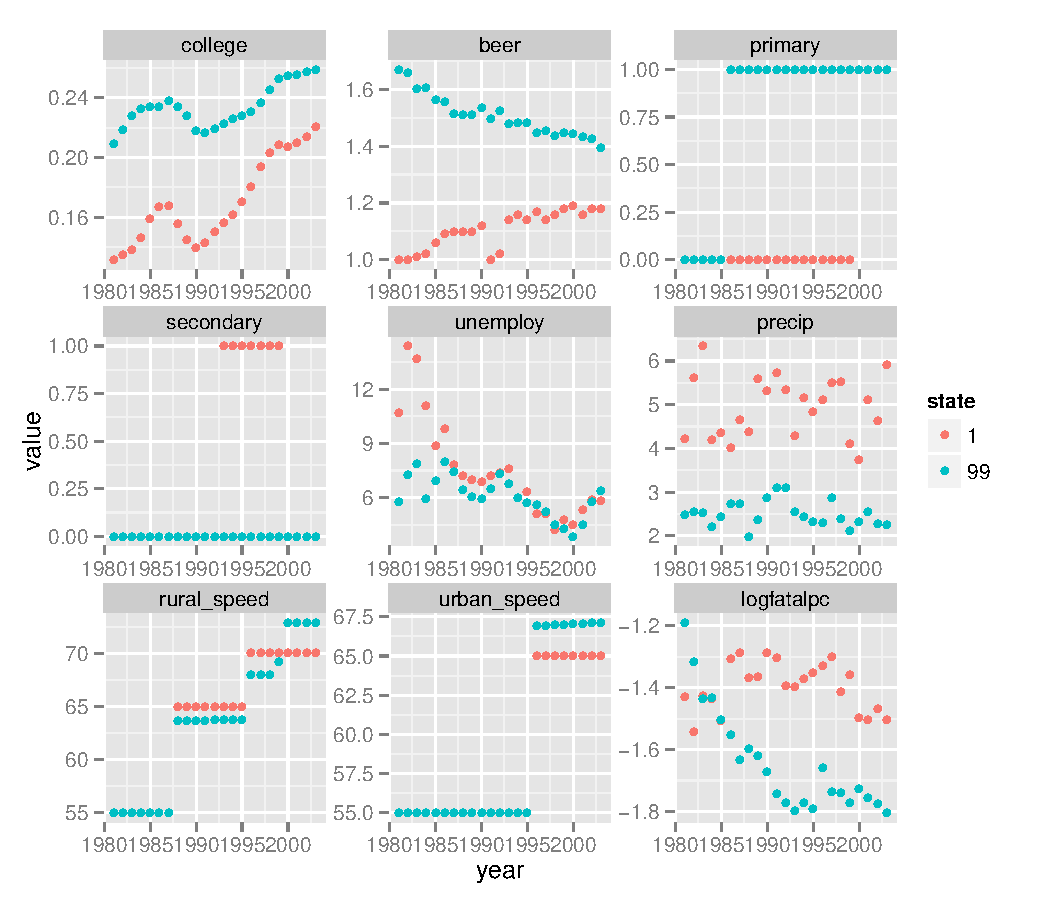
\includegraphics{img-ps2b-compareStatesFacets.pdf}
\caption{Trends in the covariate (and dependent) variables for the composite treatment state (99) and Alabama (1)}
\label{fig:a22}
\end{center}
\end{figure}


\section{Part B: Synthetic Controls}

\subsection{II: Why synthetic controls?}

\paragraph{Unsweet Home Alabama:}
We saw earlier the difficulties in selecting an exact counterfactual match for implementing differences in differences type selection on unobservables techniques.  While Alabama would appear on face value to be a good match (based on having similar outcomes in the year prior to treatment) we saw that this was coincidental and that the covariates are not a good match to the composite treatment state.  Synthetic control methods are motivated by producing a ``better" match by combining (synthesizing) multiple control states in a weighting scheme to create a composite control state with better match of the important covariates and dependent variable than any particular control state.  

\paragraph{Dr. Synth-love, or how I learned to stop worrying and love econometrics:}
Synthetic controls have a multi-step, iterative process for developing weighting factors to apply to control states for construction of a composite control state.  The goal is to identify a weighting matrix $V$ that minimizes the distance between the treatment covariates with the weighted control unit.  The steps are:

\begin{enumerate}
\item{step1...NOTE: fill out this section :)}
\end{enumerate}


\paragraph{Synthesizing control:} The process of creating a synthetic control unit involves 2 steps in the Synth package on [R].  First is specifying the form of the model in a ``data prep" step.  This is then passed to the synthetic control function to attempt implementing the algorithm described above.  In practice we found that errors arise when predictors are included that do not have variation in the mean values among the control units.  We used an additive process (adding more and more predictor covariates in the specification) to test whether there is variation.  A sub-finding is that the computational intensity increases as covariates are added.  This is a relatively small dataset but it is possible that this method could become computationally difficult with large datasets and many covariates.  After the process of adding we found that there is variation in all the potentially meaningful covariates except rural and urban speed limits.  Since speed limits were constant throughout the sample before 1986 they cannot be included in the synthetic controls specification.  

\section{Appendix: Code Listings}

\lstinputlisting{../util/are213-func.R}

\end{document}
